\documentclass[../thesis.tex]{subfiles}

\begin{document}

\chapter{Accidentals rate and DMC efficiency}
\label{chap:accDMC}

These two quantities depend on the rate of uncorrelated physics events, or \emph{singles.} The accidentals rate is determined by the probability of two singles occurring in the same coincidence window, while the efficiency of the decoupled multiplicy cut (DMC) is similarly based on the chance of one or more singles occurring within a certain distance in time from the delayed event.\footnote{IBDs and correlated backgrounds also contribute to the inefficiency of the DMC, but the effect is negligible given the vast disparity in rates between singles and correlated events.}

\def\Emin{\ensuremath{E_\mathrm{min}}}
\def\Emax{\ensuremath{E_\mathrm{max}}}
\def\Rs{\ensuremath{R_\mathrm{s}}}

Let $\Rs(\Emin, \Emax)$ be the rate of singles whose reconstructed energy lies between \Emin\ and \Emax. To be precise, \Rs\ is the \emph{true physical rate} of all \emph{muon-uncorrelated} processes that produce such singles. Naively, one could attempt to calculate \Rs\ by counting all non-muon-vetoed triggers in $(\Emin, \Emax)$ and dividing by the veto-corrected DAQ livetime. However, the rate will then be overestimated due to the inclusion of triggers from correlated events, and, likewise, the predicted accidentals spectrum will be distorted.

Instead, the correct approach is to apply an isolation cut (in time) to ensure a clean sample of true singles. A correction must then be applied for the efficiency of this cut. Once \Rs\ has been obtained in this way, calculation of the accidentals rate and DMC efficiency is a straightforward application of Poisson statistics. We now describe the calculation from end to end.

\section{Singles selection}
\label{sec:singsel}

We begin with a sample of singles, consisting of events that meet the following cuts:

\begin{comment}
  This is the current state of the code:
\begin{enumerate}
\item Not a flasher or forced trigger.
\item Not a muon.
\item AdSimple energy of at least 0.7~MeV.
\item No other events passing cuts 1-3 within time window $\pm t$.
\item Not in a muon veto window.
\end{enumerate}
Below is what it should be. Why the difference? XXX Gotta correct for the lack-of-muon-vetoing-of-other in dmcEffSingles??? Or enhance the SinglesSelector to also pull events from ClusterTree, in case the ``extra'' is vetoed (YES, THIS)? We really need to think about whether the events we're ``isolating from'' are in the same class as ``this event''. If so thend our cuts look like(?):
\end{comment}

\begin{enumerate}
\item Not a flasher or forced trigger.
\item Not in a muon veto window.
\item AdSimple energy of at least 0.7~MeV.
\item Charge of less than 3000 p.e. (i.e., not a ``pre-muon'')
\item No other events passing cuts 1-4 within time window $\pm t$.
\end{enumerate}

The muon veto cuts need not be the same as those used in the IBD selection, as long as they are sufficiently stringent so as to remove muon-correlated backgrounds. (In practice, we use the nominal LBNL muon veto.) Likewise, $t$ can be chosen arbitrarily, provided that it is long enough to remove correlated triggers and short enough to provide sufficient statistics. As currently implemented, a value of $t = 1$ms is used. This is a conservative choice; other analysis groups have successfully used values more than 50\% shorter.

\def\Rplu{\ensuremath{R_\mathrm{+}}}
\def\Rpro{\ensuremath{R_\mathrm{p}}}
\def\Rdel{\ensuremath{R_\mathrm{d}}}
\def\Rsub{\ensuremath{R_\mathrm{\lambda}}}
\def\Nplu{\ensuremath{N_\mathrm{+}}}
\def\Npro{\ensuremath{N_\mathrm{p}}}
\def\Ndel{\ensuremath{N_\mathrm{d}}}
\def\eisol{\ensuremath{\epsilon_\mathrm{i}}}
\def\emu{\ensuremath{\epsilon_\mathrm{\mu}}}

\section{Isolation cut efficiency}
\label{sec:isolcuteff}

Let us define a \emph{muon-like} event as an AD trigger with charge of at least
3000 p.e. (about 18~MeV).\footnote{It would be simpler to define a muon-like
  event directly in terms of energy instead of charge, but we use 3,000 p.e. for
  consistency with the historical LBNL analysis. Also, we don't call these
  events ``muons'', as 3,000 p.e. is not necessarily the definition of an AD
  muon used in the IBD selection.} Then a \emph{sub-muon} event is one with
reconstructed energy of at least 12~MeV, but not enough charge to be muon-like.
A \emph{prompt-like} event has energy of 0.7--12~MeV, a \emph{delayed-like}
event 6-12~MeV, and, finally, we define a \emph{prompt-plus} event as one that
is has either prompt-like or a sub-muon The sample described in the preceding
section consists of prompt-plus singles.

Similarly, we define the \emph{prompt-like rate} \Rpro\ as $\Rs(0.7, 12)$, the \emph{delayed-like rate} \Rdel\ as $\Rs(6, 12)$, the \emph{sub-muon rate} \Rsub\ as $\Rs(12, \infty)$ (up to the muon-like charge threshold), and the \emph{plus-like rate} \Rplu\ as $\Rpro + \Rsub$. Similarly, the raw event counts in our sample are \Npro, etc. To complete this round of definitions, let \eisol\ be the isolation cut efficiency, \emu\ the muon cut efficiency (for the singles selection), and $T$ be the raw DAQ livetime of the sample.

As a starting point, we have the following identity:
\begin{equation}
  \label{eq:ident0}
  \Nplu = \emu \eisol \Rplu T,
\end{equation}
in which \emu\ and $T$ are known, and \eisol\ and \Rplu\ are not.

In addition, the Poisson distribution implies that
\begin{equation}
  \label{eq:ident1}
  \eisol = e^{-2\Rplu t}.
\end{equation}
This is simply the probability of observing zero plus-like events in a time window of length $t$. The factor of 2 arises from the fact that an empty window must exist both \emph{before and after} the event.

Combining these two equations and eliminating \eisol, we have:
\begin{equation}
  \Nplu = \emu e^{-2\Rplu t} \Rplu T,
\end{equation}
which, after some rearrangement, gives:
\begin{equation}
  (-2 \Rplu t) e^{-2 \Rplu t} = - \frac{2 \Nplu t}{\emu T}.
\end{equation}
This equation takes the form $we^w = z$, which cannot be solved for $w$ (or, in our case, \Rplu) using elementary functions. Instead we employ the Lambert $W$ function, defined as the inverse of the map $w \mapsto we^w$ (that is, $W(we^w) = w$). As shown in Fig.~\ref{fig:lambertW}, the $W$ function has two branches. We know that, for a 1~ms isolation window, $\Rplu t \ll 1$, implying that the correct choice is the upper branch $W_0$. Then
\begin{equation}
  \Rplu = -\frac{1}{2t}\, W_0 \left(-\frac{2\Nplu t}{\emu T}\right)
\end{equation}

\begin{figure}
  \centering
  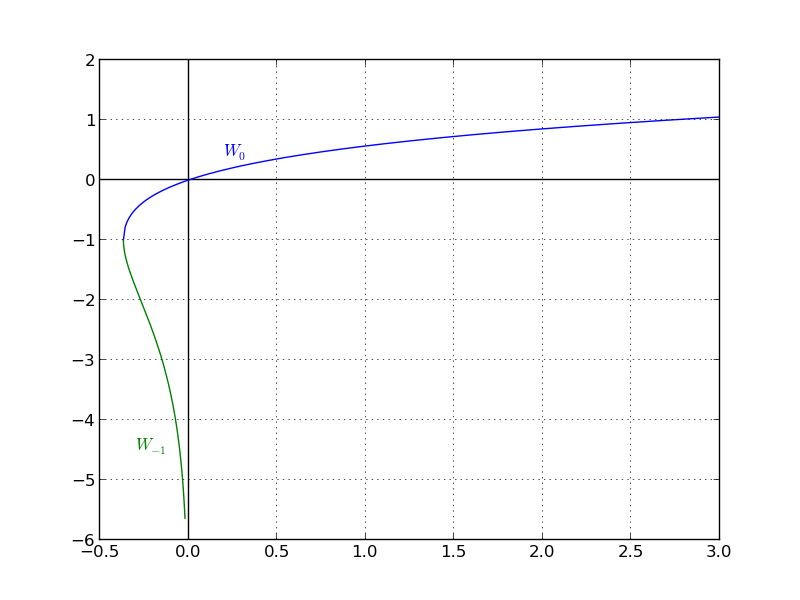
\includegraphics[scale=0.7]{../images/lambertW.png}
  \caption{The two branches of the Lambert $W$ function}
  \label{fig:lambertW}
\end{figure}

Finally, inserting this into Eq.~\ref{eq:ident0}, we obtain the isolation cut efficiency:
\begin{equation}
  \eisol = \exp W_0 \left( -\frac{2\Nplu t}{\emu T} \right).
\end{equation}

\section{Singles rates}
\label{sec:singratescalc}

Once the isolation cut efficiency is known, it is trivial to calculate the prompt- and delayed-like singles rates:
\begin{equation}
  \Rpro = \frac{\Npro}{\eisol \emu T},\qquad
  \Rdel = \frac{\Ndel}{\eisol \emu T},
\end{equation}
and so on.

\section{DMC efficiency}
\label{sec:dmceffcalc}

\def\edmc{\ensuremath{\epsilon_\mathrm{m}}}

In order for an IBD candidate to satisfy the decoupled multiplicity cut, there must be no delayed-like triggers in the 200~$\mu$s following the delayed event, and no extra plus-like events\footnote{Formerly, in the LBNL analysis, only extra \emph{prompt}-like events would lead to a DMC rejection. In order to eliminate the double neutron background, ``prompt-like'' was later changed to ``plus-like''.} in the 400~$\mu$s prior to the delayed event. More formally,
\begin{align}
  \edmc &= P(0; \Rplu \cdot 2\tau)\;P(0; \Rdel \cdot \tau) \nonumber \\
        &= \exp [-(2\Rplu\tau + \Rdel\tau)],
\end{align}
where $\tau$ = 200~$\mu$s.

\section{Accidentals rate}
\label{sec:accratecalc}

An accidental event, in order to enter the IBD selection, must pass the DMC, as with any other IBD candidate. Since the DMC is ``centered'' on the delayed event of the pair, it is simplest to calculate the accidentals rate by similarly ``centering'' the calculation on the delayed event.

Given an uncorrelated delayed-like trigger, we can calculate the probability that it forms an accidental IBD candidate. This is the product of four probabilities, where the specified time intervals are defined relative to the delayed event:

\begin{enumerate}
\item That exactly one prompt-like event occurs in [-200, 0]~$\mu$s.
\item That no sub-muon events occurs in [-200, 0]~$\mu$s.
\item That no plus-like (prompt-like or sub-muon) events occur in [-400, -200]~$\mu$s.
\item That no delayed-like events occur in [0, 200]~$\mu$s.
\end{enumerate}

\def\Racc{\ensuremath{R_\mathrm{acc}}}

The accidentals rate is then simply the product of these probabilities with the delayed-like singles rate:
\begin{align}
  \Racc &= \Rdel P(1; \Rpro \cdot \tau)\;P(0; \Rsub \cdot \tau)\;P(0; \Rplu \cdot \tau);P(0; \Rdel \cdot \tau) \nonumber \\
        &= \Rdel\,\Rpro\tau e^{-\Rpro\tau}\,e^{-\Rsub\tau}\,e^{-\Rplu\tau}\,e^{-\Rdel\tau}
\end{align}

Note that this calculation incorporates the inefficiency of the DMC (but not of the muon veto cut). By convention, the oscillation fitter expects background rates to be provided as ``theoretical'' rates, that is, the rate expected if all cuts were perfectly efficient. Internally, the fitter multiplies these rates by the DMC and veto efficiencies. Therefore, we must divide out the DMC efficiency when providing the accidentals rate to the fitter:
\begin{equation}
  \Racc' = \frac{\Racc}{\edmc}.
\end{equation}

\section{Conclusions}
\label{sec:accdmcconcl}

The most difficult and subtle part of this calculation is the efficiency of the isolation cut. I'm still not convinced that some circular logic isn't lurking in my derivation.

\end{document}